%Nous utilisons une puce atomique pour produire un gaz ultra-froid d’atomes de rubidium 87. (cf {??}) Les atomes sont dans l’état étiré $|F=2, m_F=2\rangle$. Un champ magnétique longitudinal uniforme de $B_0 = 3,36 ~\mathrm{G}$ est appliqué.

%Le piégeage transverse est assuré par trois microfils parallèles déposés sur la puce. Ces fils portent des courants alternatifs modulés à $400$ MHz. Cette configuration supprime les défauts dus à la rugosité des fils. Elle permet aussi de contrôler indépendamment les confinements longitudinal et transverse~\cite{PhysRevLett.98.263201}.

%Les atomes sont piégés à $7\,\mu$m de la surface de la puce et à $15\,\mu$m des fils. Cela donne un confinement transverse fort. Ce potentiel transverse est bien décrit par un piège harmonique. Sa fréquence est $\omega_\perp/2\pi = 2{,}56$ kHz pour les données présentées ici.

Nous produisons un gaz ultra-froid d’atomes bosoniques de $^{87}$Rb dans l’état $|F=2,m_F=2\rangle$ à l’aide d’une puce atomique. En plus d’un champ magnétique longitudinal homogène $B_0 = 3{,}36$G, le confinement transverse est assuré par trois microfils parallèles déposés sur la puce (représentés en bleu sur la Fig.\ref{fig:setup}(a)) parcourus par des courants alternatifs modulés à $400$MHz. Cette configuration permet d’éliminer les effets de rugosité des fils et d’ajuster indépendamment les confinements longitudinal et transverse \cite{PhysRevLett.98.263201}. Les atomes sont piégés à $7\mu$m de la surface de la puce et à $15~\mu$m des fils, ce qui permet un confinement transverse intense. Le potentiel transverse est bien décrit par un potentiel harmonique de fréquence $\omega_{\perp}/2\pi = 2{,}56$~kHz dans les données présentées ici.

%Par évaporation radiofréquence, nous refroidissons le gaz jusqu'à une température de $T = 100~\mathrm{nK}$. Le potentiel chimique est $\mu/k_B = 45~\mathrm{nK}$. Ainsi, on a $\mu/(\hbar\omega_\perp) = 0,4$ et $k_B T/(\hbar\omega_\perp) = 0,8$. Le gaz entre alors dans le régime unidimensionnel.

Un refroidissement évaporatif par radiofréquence nous permet d’obtenir un nuage atomique à une température d’environ $T = 100$~nK, pour un potentiel chimique $\mu / k_B = 45$~nK. Avec ces paramètres, on obtient les rapports $\mu / (\hbar \omega_{\perp}) = 0{,}4$ et $k_B T / (\hbar \omega_{\perp}) = 0{,}8$, ce qui place le gaz dans le régime unidimensionnel. Le couplage effectif en 1D pour des atomes dans l’état fondamental transverse est donné par $g = 2 a_{3D} \hbar \omega_{\perp}$ \cite{PhysRevLett.81.938}, où $a_{3D} = 5{,}3$nm est la longueur de diffusion tridimensionnelle du $^{87}$Rb\cite{PhysRevLett.89.283202}. Des détails supplémentaires sur l’expérience sont disponibles dans \cite{duboistel-04749900}.

%Le couplage effectif en 1D est donné par $g = 2 a_{3D} \hbar \omega_\perp$~(??), avec $a_{3D} = 5.3~\mathrm{nm}$, la longueur de diffusion en 3D pour le rubidium 87~(cf {??}).Le paramètre sans dimension de Lieb est $\gamma = mg / (\hbar^2 n_0)$, avec $n_0$ la densité linéaire. Il varie entre $0,004$ et $0,007$. La température vérifie $T \ll n_0^{3/2} \sqrt{\hbar^2 g / m}/k_B$, ce qui place le gaz dans le régime de quasi-condensat~(cf {??}).

%Le piégeage longitudinal est assuré par quatre fils supplémentaires. Ces fils sont placés de part et d’autre des trois microfils transverses (voir Fig.~??(a)). Ils sont éloignés du centre de la puce. Le potentiel longitudinal est alors bien approché par une série de polynômes : $V(x) = \sum_i a_i x^i$.Nous ajustons les courants dans ces fils pour annuler les termes linéaire, quadratique et cubique ($a_1$, $a_2$, $a_3$). Le terme dominant est alors le terme quartique : $V(x) = a_4 x^4$.Ce type de piège crée une densité atomique quasi homogène sur une grande longueur. C’est important pour notre étude, car le protocole de coupure bipartite suppose un système semi-infini.Un exemple de profil de densité dans un tel potentiel est donné en gris sur la Fig.~\ref{fig:setup}(b). La densité linéaire $n_0$ reste constante à $10\%$ près sur une longueur d’environ $250\,\mu$m.

%Pour créer la coupure initiale, nous utilisons une méthode de sélection spatiale~(Part {??}). %Nous éclaireons le bord gauche du nuage avec un faisceau quasi résonant. Ce faisceau est proche de la transition $F=2 \rightarrow F'=3$ de la raie D2. Il est perpendiculaire à l’axe longitudinal $x$.Les atomes exposés à ce faisceau subissent une pression de radiation. Une exposition de $30\,\mu$s (environ 15 cycles d’absorption/réémission) suffit pour qu’ils quittent le piège. Le faisceau est façonné à l’aide d’un dispositif à micro-miroirs (DMD) pour ne viser qu’un bord du gaz.

%Cette méthode crée une frontière nette entre une région vide et un gaz homogène. Cette netteté est surtout limitée par la résolution de l’image, de l’ordre du micromètre. L’effet de réabsorption des photons diffusés peut aussi réduire la netteté. Pour l’atténuer, on détune le faisceau de $15 ~\mathrm{MHz}$ par rapport à la transition D2.

%Le profil de densité après cette sélection est montré en jaune dans la Fig.~\ref{fig:setup}. Le gaz est alors homogène à $10\%$ près sur environ $250\,\mu$m.

%Après cette préparation, nous relâchons le confinement longitudinal tout en maintenant le piège transverse. La frontière initiale s’élargit avec le temps. Nous suivons cette dynamique en enregistrant les profils de densité $n(x;t)$ à différents temps d’évolution.





Le paramètre sans dimension de Lieb $\gamma = m g / (\hbar^2 n_0)$, avec $n_0$ la densité linéique, se situe dans l’intervalle $[0{,}4,0{,}7] \times 10^{-2}$, tandis que la température satisfait l’inégalité $T \ll n_0^{3/2} \sqrt{\hbar^2 g / m} / k_B$. Ainsi, les gaz obtenus se trouvent profondément dans le régime de quasicondensat \cite{PhysRevLett.91.040403}.

Le piégeage longitudinal est assuré par des courants continus circulant dans quatre fils placés de part et d’autre des trois microfils de confinement transverse, comme illustré sur la Fig.\ref{fig:setup}(a). Étant donné que ces fils sont situés loin du centre du nuage atomique, le potentiel longitudinal peut être développé en série polynomiale : $V(x) = \sum_i a_i x^i$. Les quatre premiers coefficients $a_i$ peuvent être ajustés en modulant les courants dans ces fils. Il est ainsi possible d’annuler les termes linéaire, quadratique et cubique ($a_1 = a_2 = a_3 = 0$), de sorte que le terme dominant du potentiel soit quartique : $V(x) = a_4 x^4$. Une telle forme de potentiel permet d’obtenir une densité atomique quasi homogène sur une région relativement étendue, condition essentielle à l’étude de dynamiques hors équilibre telles que le protocole de coupure bipartite, qui suppose un système semi-infini. Un exemple de profil de densité linéique obtenu dans ce potentiel quartique est représenté en gris sur la Fig.\ref{fig:setup}(b). La densité linéique $n_0$ y reste constante à $10\%$ près sur une distance d’environ $250~\mu$m.

Pour réaliser expérimentalement une bipartition initiale nette, nous utilisons la méthode de sélection spatiale introduite dans \cite{PhysRevLett.133.113402}. Une partie du nuage, initialement dans un état stationnaire global dans le piège quartique, est illuminée à son extrémité gauche par un faisceau lumineux quasi résonant avec la transition $F=2 \rightarrow F'=3$ de la raie D2, se propageant perpendiculairement à l’axe $x$. Les atomes exposés subissent une pression de radiation : après $30~\mu$s d’illumination, correspondant à environ 15 cycles absorption/réémission, ces atomes acquièrent une énergie suffisante pour quitter le piège. Le faisceau est façonné spatialement à l’aide d’un dispositif à micromiroirs numériques (DMD) afin de ne cibler qu’un bord du gaz. Ce protocole produit une frontière nette entre une région vide et un gaz quasi homogène, rendue possible par l’utilisation du piège quartique. La résolution de cette coupure est limitée principalement par la résolution du système d’imagerie (quelques microns). L’éventuelle réabsorption des photons diffusés par les atomes non illuminés est réduite en désaccordant le faisceau pousseur de $15$MHz par rapport à la transition D2. Un exemple de profil de densité après application de ce protocole est illustré en jaune sur la Fig.\ref{fig:setup}(b).

Une fois la coupure réalisée, le confinement longitudinal est supprimé tout en maintenant le confinement transverse. La frontière initialement abrupte s’élargit au cours du temps. Cette dynamique est étudiée par imagerie, en enregistrant les profils de densité longitudinale $n(x,t)$ pour différentes durées d’évolution $t$.

\begin{figure}[!htb]
\centering
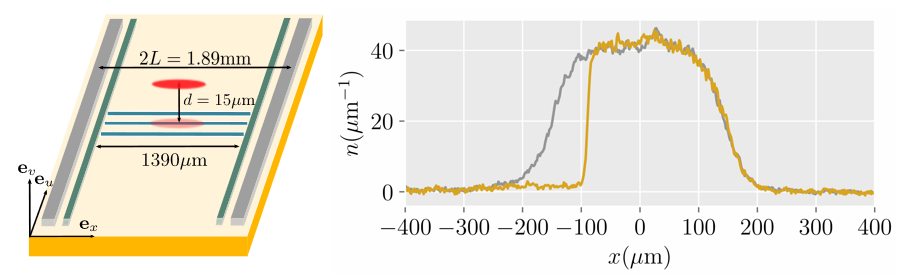
\includegraphics[width=0.90\linewidth]{Atom_chip.png}
\caption{(a) Schéma de la puce atomique. Les $3$ fils bleus assurent le confinement transverse, les $4$ autres fils (gris) génèrent le potentiel longitudinal. Le nuage atomique, représenté par une ellipse rouge, est piégé à $12~\mu$m au-dessus des fils. (b) Profils de densité linéique extraits par imagerie par absorption. En gris : gaz piégé dans un potentiel quartique. En jaune : après application du faisceau pousseur pendant $30~\mu$s, suivi d’un temps de vol de $1$~ms.}
\label{fig:setup}
\end{figure}
